\chapter{有限元素法}

\begin{figure}[hbt!]
\begin{center}
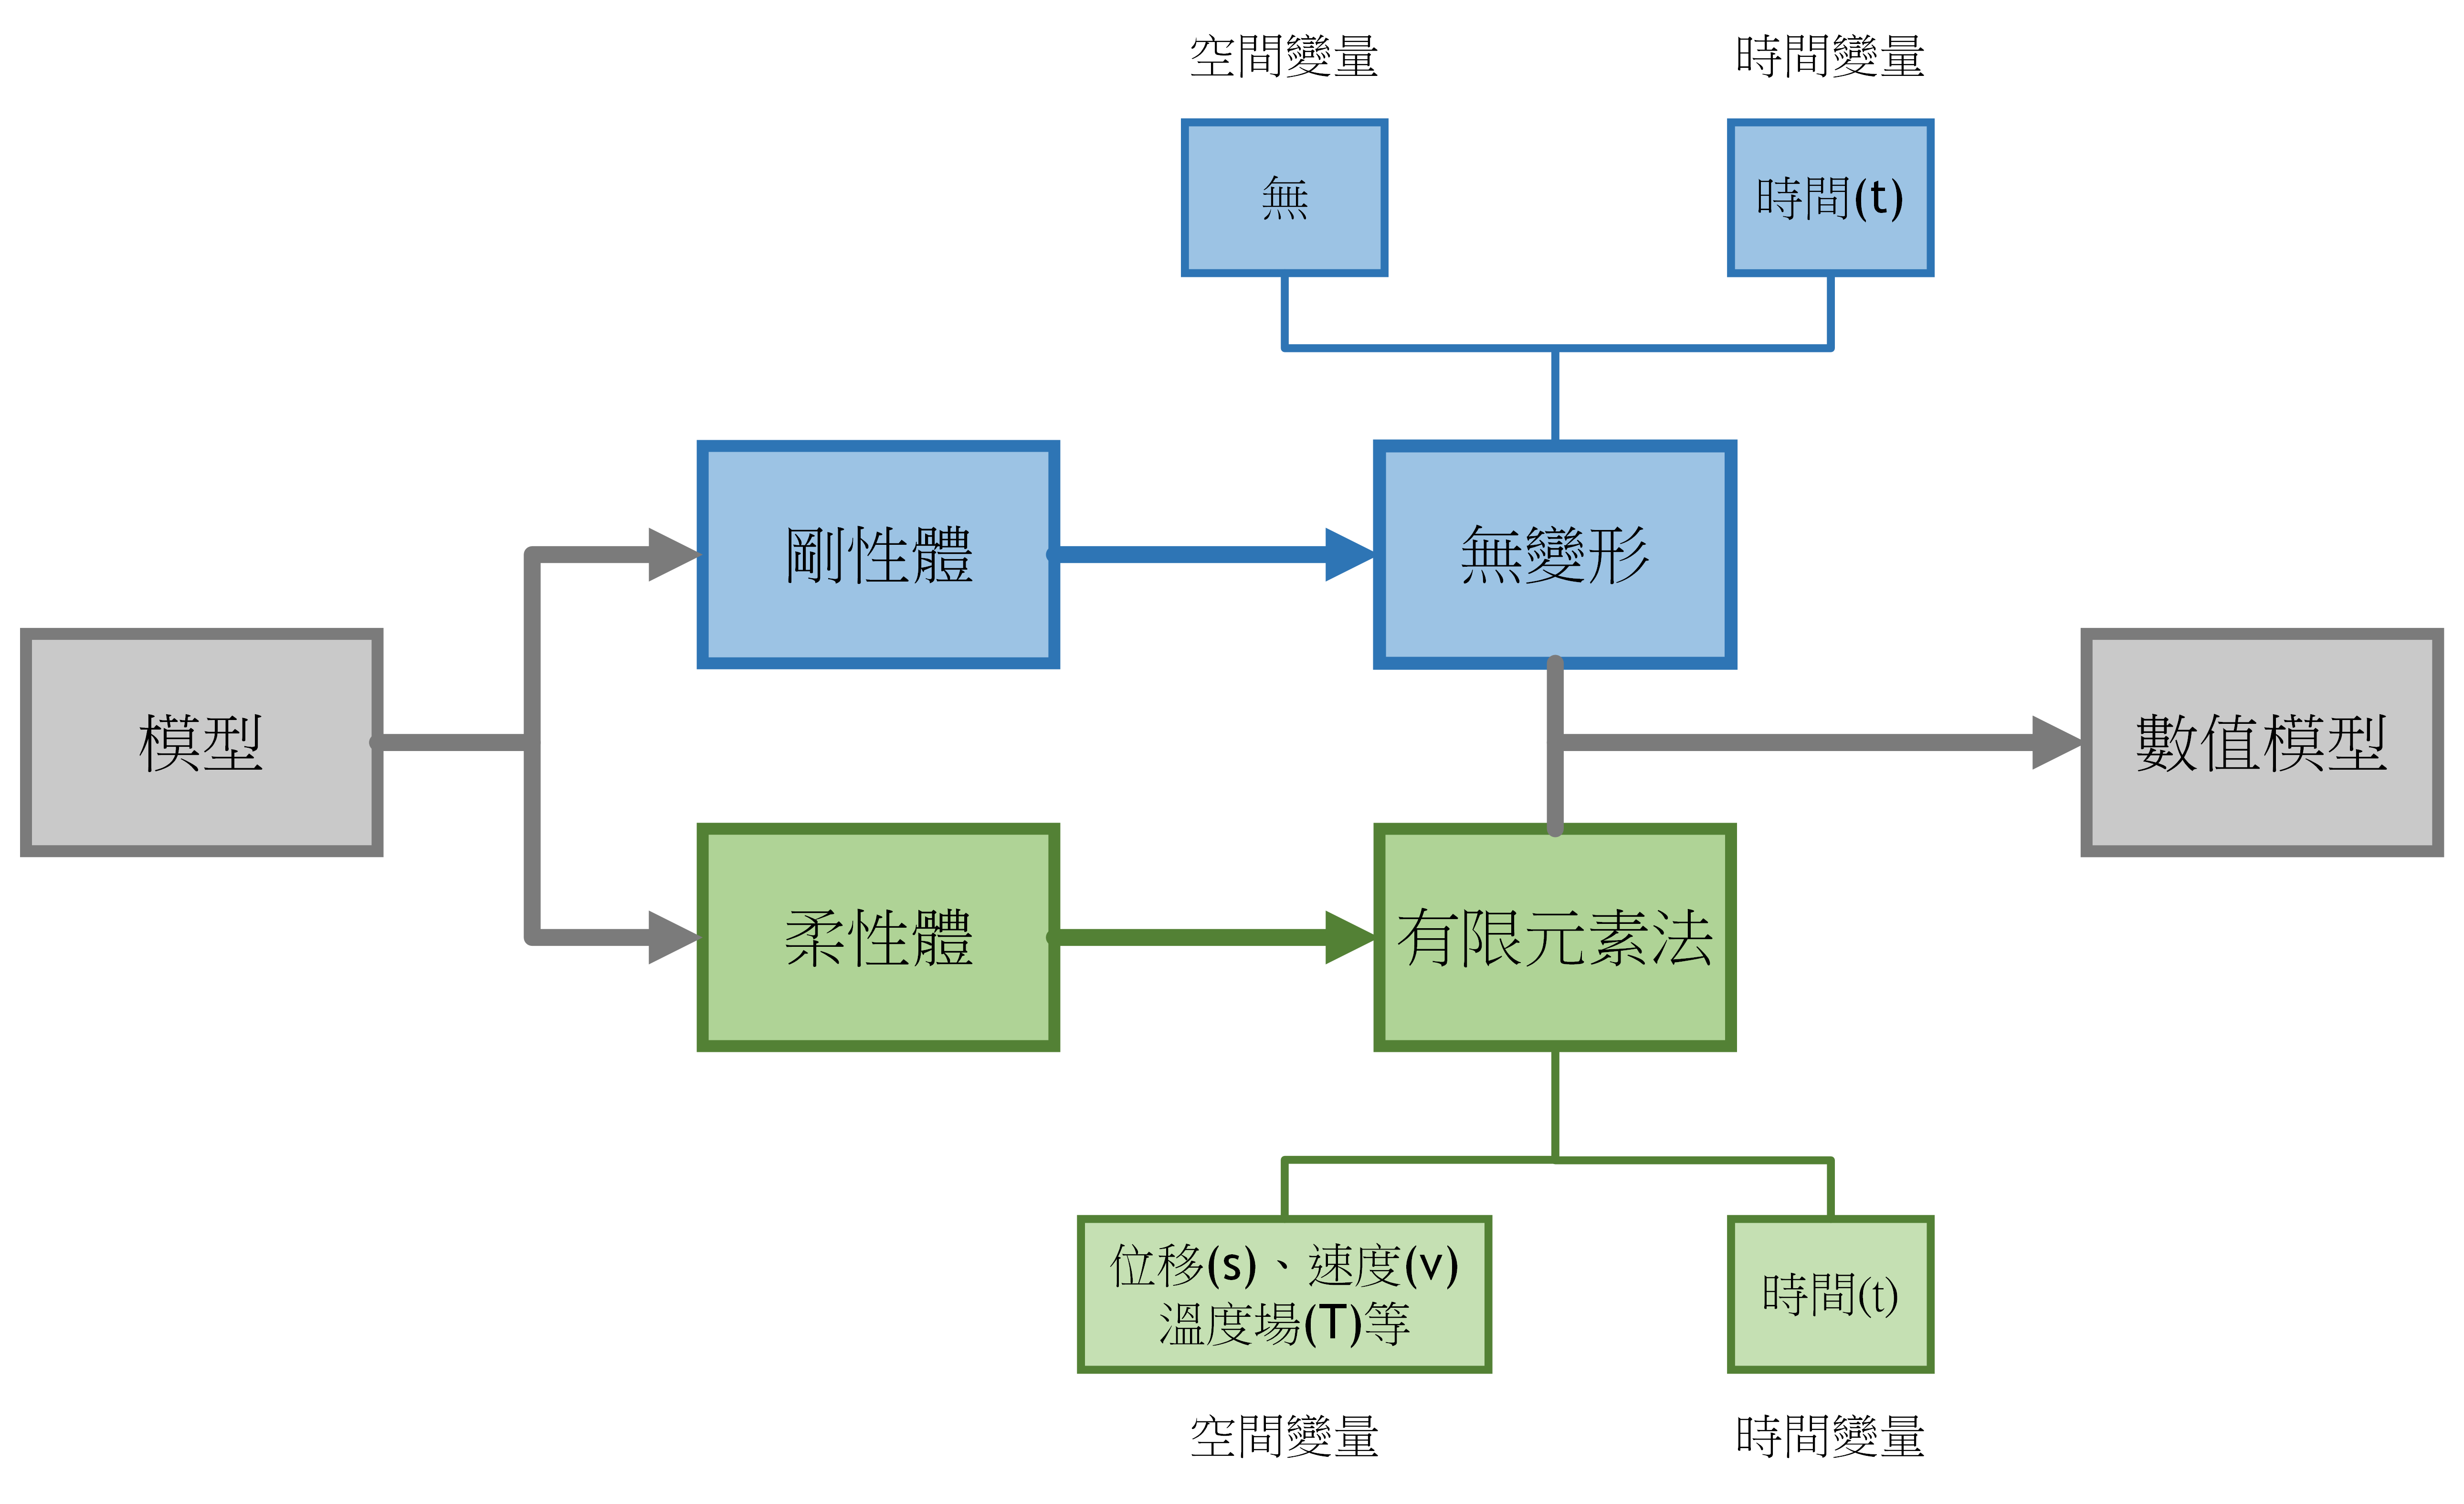
\includegraphics[width=14cm]{有限元素法}
\caption{\Large 有限元素法流程及架構}\label{有限元素法}
\end{center}
\end{figure}
用於求解偏微分方程或積分方程組數值求解,將大型物理系統細分為更小、更簡單的部分,稱為有限元,通過在空間維度上進行特定的空間離散化簡化連續變量的複雜性,有限元素法通過最小化關聯的誤差函數,使用來自變異演算的變異方法來近似求解,來實現用於複雜的工程結構或物理系統的行為。\\
通常用在具有多種變量的模型上,在分析之前通常加設物理為剛體,剛體狀態下的模擬較為可控並且只擁有時間變量,所以使用常微分方程及可計算。\\
而柔性體則會因為受力情況的不同而產生多種變量,才需要利用偏微分方程求解,對物體進行離散化並劃分網格如(圖.2.1),接著代入方程計算,此動作稱為有限元素法。\\
\newpage
%---------------------第二章/基本概念及假設假定-------------------------%
\section{基本概念}

\begin{figure}[hbt!]
\begin{center}
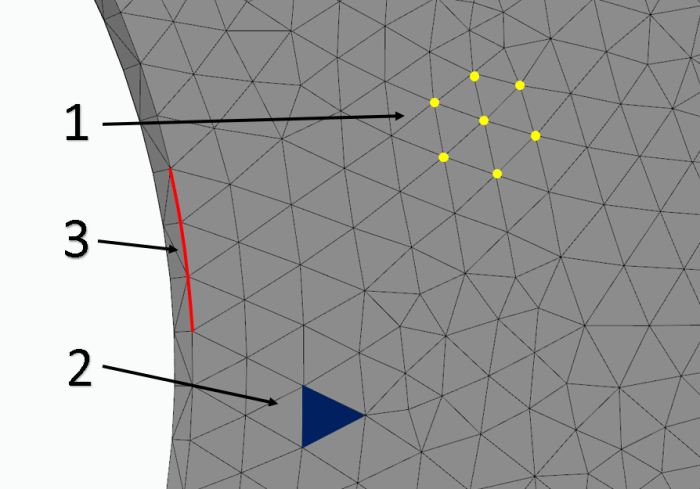
\includegraphics[width=14cm]{有限元素法介紹}
\caption{\Large 基本概念}\label{有限元素法介紹}
\end{center}
\end{figure}

\begin{enumerate}
\item 節點:每個元素的角落或中心點,用於連接元素之間的邊界條件和解決方程,如(圖.2.1)上所箭頭1指示。
\item 元素:通常由三角形或者四邊形等形成的區域結構,如(圖.2.1)上箭頭2所指示。
\item 邊界條件:存在於物理系統邊界上的約束及負荷力,模擬實際情況下的條件約束和外界影響,如(圖.2.1)上箭頭3所指示。
\item 自由度: 節點上變量的個數,例如位移的節點自由度為3,表示單個節點擁有三個坐標方向的位移,又例如熱分析時節點自由度為1,表示某個節點處的溫度。
\item 網格:由數個元素經由節點連接所組成,用以表示在需求解的區域上。
\item 變形:系統在外力的影響下發生的形變,經過分析後計算每個元素的變形及變形之間的相互引響預測整得系統的變形及應力、各種參數的分布。
\item 離散化:將物理系統或結構等連續變量通過計算轉換為數格元素的過程,目的在於減化數據,減少連續變量的複雜性,便於處理及分析。關於公式及步驟會因為模型或問題的類型不同而有不一樣的計算方式。
\item 材料特性:物理系統(模型)的材料性質,不同的材料其中的參數各為不同(彈性模數、蒲松比、極限強度、降伏強度等)。\
\end{enumerate}

\subsection{邊界條件}
分為兩種邊界條件,為位移值或施加力條件。

\begin{enumerate}
\item 位移邊界條件:規定了結構或邊界上的位移及變形的特定值或關係。

\begin{itemize}
\item 固定邊界條件:也稱為約束邊界條件,令特定的某些節點或自由度的位移為零,使其無法發生位移。
\item 位移約束:指定特定節點或自由度的位移值, 可以是定值或隨時間變化的函數。
\item 斜率約束:規定特定節點的自由度的位移斜率(導數),用於描述特定邊界上的傾斜或旋轉。
\end{itemize}

\item 力邊界條件:規定了結構或邊界上施加的外部力或力的分布。

\begin{itemize}
\item 負荷:施加在結構上的集中力或分布力,可以是靜態或動態負荷。
\item 壓力:施加在邊界上的或表面力,可以是均勻或非均勻的。
\item 動力學條件:施加在結構上的動態加載。
\end{itemize}
\end{enumerate}

\subsection{網格劃分基本原則}
\begin{enumerate}
\item 網格數量:將決定計算精度及規模大小,一般狀況中,網格數量增加計算精度也會跟著提升,但伴隨而來的是更大的計算量,所以在制定網格大小時應權衡兩個因素。
\item 網格疏密:在某些變化梯度較大的部位(應力集中處),需要大密集的網格,密集往個將更好反映數據變化,反之變化梯度較小的部位則用較稀疏的網格,而不同單元之間的連接則採用特殊的過度單元或多點約束等方法連接,才能更好的分配資源,兼顧計算量何計算精度。
\item 網格質量:指網格形狀的合理性,質量的好壞將直接影響計算精度,質量較差的除了造成局部的計算精度偏差甚至會直接終止計算,因此在重要部位時應該確保其擁有高品質的表現。
如果網格都是由等邊三角形、正方形、正四面體、立方六面體等組成,則求解精度可以非常接近實際值,但這種只存在於理想狀態下,實際運用卻很難做到。\
\end{enumerate}

\begin{itemize}
\item 元素質量評價指標
\end{itemize}

\begin{enumerate}
\item 單元的邊長比、面積比及體積比,理想的邊長比為1,以正三角形、正四面體、正六面體為參考基準。
\item 扭曲度:單元內部扭轉及面外的翹曲程度。
\item 疏密過渡:應力梯度方向和橫向過渡情況,應力集中部分應較為密集,則反之。
\item 節點、元素排部:合理的節點及元素有助於帶入方程式計算,可以提高求解效率,並且須注意消除重複的節點及元素。
\end{enumerate}
下列(圖.2.2)至(圖.2.5)為網格疏密不同造成的分析差\

\begin{figure}[htbp]
  \centering
  \begin{minipage}{0.45\textwidth}
    \centering
    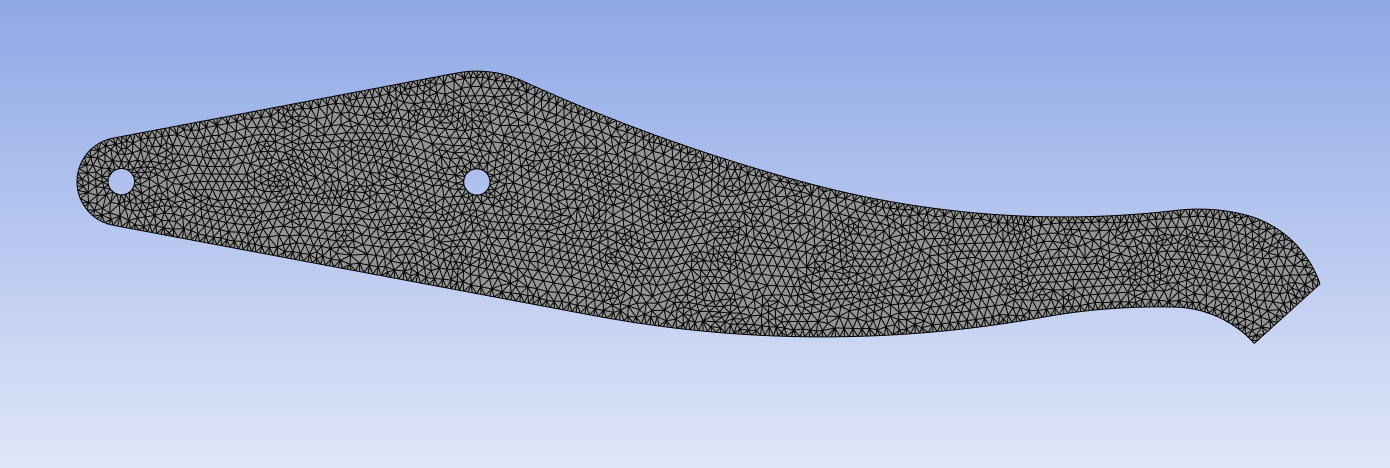
\includegraphics[width=\textwidth]{網格1mm-1}
    \caption{較密網格}
    \label{網格1mm-1}
  \end{minipage}
  \hfill
  \begin{minipage}{0.45\textwidth}
    \centering
    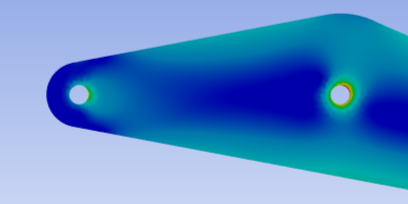
\includegraphics[width=\textwidth]{網格1mm-2}
    \caption{較密網格所得應力雲圖}
    \label{網格1mm-2}
  \end{minipage}
  
  \vspace{0.75cm} % 調整垂直間距
  
  \begin{minipage}{0.45\textwidth}
    \centering
    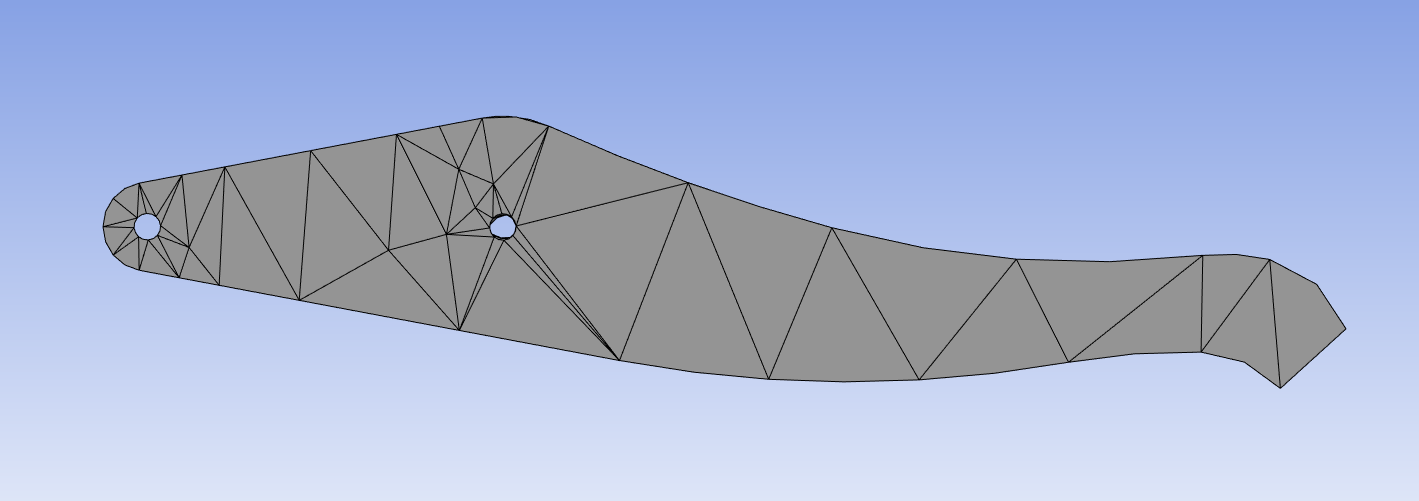
\includegraphics[width=\textwidth]{網格50mm-1}
    \caption{較粗網格}
    \label{網格50mm-1}
  \end{minipage}
  \hfill
  \begin{minipage}{0.45\textwidth}
    \centering
    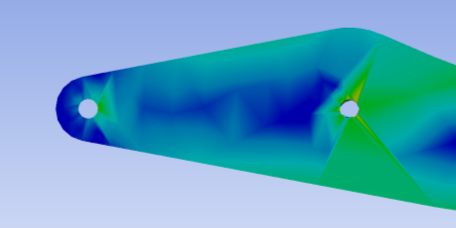
\includegraphics[width=\textwidth]{網格50mm-2}
    \caption{較粗網格所得應力雲圖}
    \label{網格50mm-2}
  \end{minipage}
\end{figure}
\newpage
%--------------------------第二章/有限元計算公式--------------------------%
\section{有限元計算公式}
對於有限元素法代入模型的各種問題求解,以下有著幾種常用計算公式,分別對三角形元素和四角形元素及各式運動方程進行計算。
%---------------------{應力計算}---------------------%
\begin{itemize}
\item 應力計算
\end{itemize}

\begin{enumerate}
\item 對於三角形元素而言,其計算方法如下:\
\[
\begin{aligned}
\sigma x=&\left( \dfrac{1}{\Delta }\right) \times \left[ \sigma _{1}\times \left( y_{2}-y_{3}\right) +\sigma _{2}\times \left( y_{3}-y_{1}\right) +\sigma _{3}\times \left( y_{1}-y_{2}\right) \right]\\
\sigma y=&\left( \dfrac{1}{\Delta }\right) \times \left[ \sigma _{1}\times \left( x_{3}-x_{2}\right) +\sigma _{2}\times \left( x_{1}-x_{3}\right) +\sigma _{3}\times \left( x_{2}-x_{1}\right) \right]\\
\tau xy=&\left( \dfrac{1}{\Delta }\right) \times \left[ \tau _{1}\times \left( x_{3}-x_{2}\right) +\tau _{2}\times \left( x_{1}-x_{3}\right) +\tau _{3}\times \left( x_{2}-x_{1}\right) \right]\\
\end{aligned}
\]
其中,σx, σy, τxy 分別表示在 x, y 方向上的正應力和剪應力,σ1, σ2, σ3 表示每個節點上的應力,τ1, τ2, τ3 表示每個節點上的剪應力,Δ 表示三角形單元的面積。\

\item 對於四邊形元素而言,其計算方法如下:\
\[
\begin{aligned}
\sigma _{x}=&\left( \dfrac{1}{4t}\right) \times \left[ \sigma _{1}\times \left( y_{4}-y_{2}\right) +\sigma _{2}\times \left( y_{1}-y_{3}\right) +\sigma _{3}\times \left( y_{2}-y_{4}\right) +\sigma _{4}\times \left( y_{3}-y_{1}\right) \right]\\
\sigma _{y}=&\left( \dfrac{1}{4t}\right) \times \left[ \sigma _{1}\times \left( x_{2}-x_{4}\right) +\sigma _{2}\times \left( x_{3}-x_{1}\right) +\sigma _{3}\times \left( x_{4}-x_{2}\right) +\sigma _{4}\times \left( x_{1}-x_{4}\right) \right]\\
\tau xy=&\left( \dfrac{1}{4t}\right) \times \left[ \tau _{1}\times \left( x_{2}-x_{4}\right) +\tau _{2}\times \left( x_{3}-x_{1}\right) +\tau 3\times \left( x_{4}-x_{2}\right) +\tau 4\times \left( x_{1}-x_{3}\right) \right]\\
\end{aligned}
\]
其中,σx, σy, τxy 分別表示在 x, y 方向上的正應力和剪應力,σ1, σ2, σ3, σ4 表示每個節點上的應力,τ1, τ2, τ3, τ4 表示每個節點上的剪應力,t 表示四邊形單元的厚度。
\end{enumerate}

\begin{itemize}
\item 有限元素應力計算公式
\end{itemize}
\begin{enumerate}
\item 對於三角形元素而言,其計算方法如下:\
\[
\begin{aligned}
\varepsilon x=&\left( \dfrac{1}{\Delta }\right) \times \left[ \varepsilon 1\times \left( y_{2}-y_{3}\right) +\varepsilon 2\times \left( y_{3}-y_{1}\right) +\varepsilon 3\times \left( y_{1}-y_{2}\right) \right]\\
\varepsilon y=&\left( \dfrac{1}{\Delta }\right) \times \left[ \varepsilon 1\times \left( x_{3}-x_{2}\right) +\varepsilon 2\times \left( x_{1}-x_{3}\right) +\varepsilon 3\times \left( x_{2}-x_{1}\right) \right]\\
\gamma xy=&\left( \dfrac{1}{\Delta }\right) \times \left[ \gamma _{1}\times \left( x_{3}-x_{2}\right) +\gamma _{2}\times \left( x_{1}-x_{3}\right) +r_{3}\times \left( x_{2}-x_{1}\right) \right]\\
\end{aligned}
\]\
其中,εx, εy 分別表示在 x, y 方向上的應變,γxy 表示剪應變,ε1, ε2, ε3 分別表示每個節點上的應變,γ1, γ2, γ3 表示每個節點上的剪應變,Δ 表示三角形單元的面積。\
\item 對於四邊形元素而言,其計算方法如下:\
\[
\begin{aligned}
\varepsilon _{x}=&\left( \dfrac{1}{4t}\right) \times \left[ \varepsilon _{1}\times \left( y_{4}-y_{2}\right) +\varepsilon _{2}\times \left( y_{1}-y_{3}\right) +\varepsilon _{3}\times \left( y_{2}-y_{4}\right) +\varepsilon _{4}\times \left( y_{3}-y_{1}\right) \right]\\
\varepsilon _{y}=&\left( \dfrac{1}{4t}\right) \times \left[ \varepsilon _{1}\times \left( x_{2}-x_{4}\right) +\varepsilon _{2}\times \left( x_{3}-x_{1}\right) +\varepsilon _{3}\times \left( x_{4}-x_{2}\right) +\varepsilon _{4}\times \left( x_{1}-x_{4}\right) \right]\\
\gamma xy=&\left( \dfrac{1}{4t}\right) \times \left[ \gamma _{1}\times \left( x_{2}-x_{4}\right) +\gamma _{2}\times \left( x_{3}-x_{1}\right) +\gamma 3\times \left( x_{4}-x_{2}\right) +\gamma 4\times \left( x_{1}-x_{3}\right) \right]\\
\end{aligned}
\]
其中,εx, εy 分別表示在 x, y 方向上的應變,γxy 表示剪應變,ε1, ε2, ε3, ε4 分別表示每個節點上的應變,γ1, γ2, γ3, γ4 表示每個節點上的剪應變,t 表示四邊形單元的厚度。
\end{enumerate}

\begin{itemize}
\item 有限元素動力學分析公式
\end{itemize}
\begin{enumerate}
\item 結構的運動方程:\\
在有限元素動力學分析中,結構的運動方程通常採用以下形式表示:\
\[
\begin{aligned}
\left[ M\right] \times \left\{ u''\right\} +\left[ C\right] \times \left\{ u'\right\} +\left[ K\right] \times \left\{ u\right\}=&\left\{ F\left( t\right) \right\}\\
\end{aligned}
\]
其中,[M]、[C] 和 [K] 分別表示結構的質量、阻尼和剛度矩陣,{¨u}、{˙u} 和 {u} 分別表示結構的加速度、速度和位移矢量,{F(t)} 表示結構受到的外部激勵矢量。\

\item 求解運動方程:\\
通過對運動方程進行離散化處理,可以得到結構的位移、速度和加速度的數值解。通常採用時間步進法求解運動方程,其中最常用的是 Newmark-β 方法,其求解公式如下:\
\[
\begin{aligned}
\left\{ u\left( t+\Delta t\right) \right\}=&\left\{ u\left( t\right) \right\} +\left\{ u'\left( t\right) \right\} \Delta t+\left( \dfrac{1}{2}-\beta \right) \times \left\{ u''\left( t\right) \right\} \Delta t^{2}+\beta \left\{ u''\left( t+\Delta t\right) \right\} \Delta t^{2}\\
\left\{ u'\left( t+\Delta t\right) \right\}=&\left\{ u'\left( t\right) \right\} +\left( 1-\gamma \right) \times \left\{ u''\left( t\right) \right\} \Delta t+\gamma \left\{ u''\left( t+\Delta t\right) \right\} \Delta t\\
\end{aligned}
\]
其中,β 和 γ 是時間步進法的參數,其取值需要根據求解的精度和計算效率進行權衡。\

\item 應力計算公式\
在求解結構動態響應的過程中,通常需要計算結構內部的應力分佈情況。對於有限元素動力學分析而言,常用的應力計算公式是根據結構位移和應變之間的關係推導而來的。具體來說,可以採用以下公式進行應力計算:\
\[
\begin{aligned}
\left\{ \sigma \right\}=&\left[ D\right] \times \left\{ \varepsilon \right\}
\end{aligned}
\]
其中,{σ} 和 {ε} 分別表示應力和應變矢量,[D] 表示材料的彈性剛度矩陣,其數值可以根據材料的力學性質進行計算。

\end{enumerate}

\begin{itemize}
\item 有限元素疲勞分析公式
\end{itemize}
\begin{enumerate}

\item 疲勞壽命計算公式\
在有限元素疲勞分析中,常用的疲勞壽命計算公式是基於線性累積損傷理論的公式,其表示形式如下:\\
\[
\begin{aligned}
N=\dfrac{1}{\left( \Delta ^{\sigma }/2S\right) ^{m}}\\
\end{aligned}
\]
其中,N 表示疲勞壽命,Δσ 表示應力幅值,S 表示材料的疲勞極限,m 是材料的疲勞指數,其數值可以根據材料的力學性質進行計算。\\

\item 應力計算公式\
在有限元素疲勞分析中,需要對結構的應力分佈進行計算。常用的應力計算公式是基於虛功原理推導而來的,其表示形式如下:\\
\[
\begin{aligned}
\int \left\{ \sigma \right\} T\left\{ \delta \varepsilon \right\} dV=&\int \left\{ f\right\} T\left\{ \delta u\right\} dV+\int \left\{ T\right\} T\left\{ \delta u\right\} dS\\
\end{aligned}
\]
其中,{σ} 和 {ε} 分別表示應力和應變矢量,{f} 表示結構受到的外部載荷矢量,{u} 表示結構的位移矢量,{T} 表示結構的邊界條件。\\

\item 疲勞壽命修正公式
在實際應用中,疲勞壽命計算公式需要考慮多種因素的影響,如應力比、材料強度和載荷歷史等。常用的疲勞壽命修正公式包括 Goodman、Soderberg、Walker 和 Morrow 等,其表示形式可以根據具體的應用要求進行選擇。
\end{enumerate}

\section{分析步驟}
\begin{itemize}
\item 幾何模型:透過繪圖軟體將模型畫出,將模型以數據方式在電腦裡呈現二維或三維的外觀,便於軟體將其代入且計算。
\item 離散化及元素劃分: 將物理系統或結構等連續變量通過計算轉換為數格元素的過程,對於複雜的連續變量,需先進行離散的動作,將其轉變為各個元素,此動作由分析軟體內部公式計算。
\item 導入函數並組成代數方程: 模型或問題不同,力學性質及物理方程相應的關係式(應力、應變、變形、熱傳等)也會跟著變化,因此需要根據對應的問題分別導入不同的函數,需在軟體內設定問題,讓其可以對特定問題進行求解,此動作為設計者提問,軟體負責計算。
\item 求解方程:在經過有限元素法分析後,將會在每個表面得知各元素的受力情況,設計者可以根據此數據了解到模型的受力狀態或位移及負載等相關訊息,以利於後續的設計或生產。
\end{itemize}
\newpage
